% -----------------------------------------------------------------------------
\section{Recommended Best Practices}
\label{sec:bestpractices}
% -----------------------------------------------------------------------------
\subsection{SBOL Versions}

To differentiate between major versions of SBOL, different namespaces are used.  For example, SBOL3 has the namespace \url{http://sbols.org/v3#}, while SBOL2 has the namespace \url{http://sbols.org/v2#}.  These different versions of SBOL SHOULD NOT be semantically mixed. For example, an SBOL 3.x \sbol{SubComponent} SHOULD NOT refer to an SBOL 2.x \sbol{ComponentInstance}, and, likewise, an SBOL 2.x \sbol{ComponentInstance} SHOULD NOT refer to an SBOL 1.x \sbol{DnaComponent}.

\subsection{Compliant SBOL Objects}
\label{sec:compliant}

Maintaining unique URIs for all SBOL objects can be a very challenging implementation task.  To reduce this burden, users of SBOL 3.x are encouraged to follow a few simple rules when constructing the URIs and related properties for SBOL objects.  When these rules are followed in constructing an SBOL object, we say that this object is \emph{compliant}. These rules are as follows:

Compliant URIs for \sbol{TopLevel} objects MUST conform to the following pattern:
\begin{quotation} 
\refObj{namespace}/\refObj{collection\_structure}/\refObj{displayId}
\end{quotation}

The \refObj{namespace} token itself may further decompose into \refObj{domain}/\refObj{root} tokens. The \refObj{root} and \refObj{collection\_structure} tokens may optionally be omitted; alternatively, they may consist of an arbitrary number of delimiter-separated layers. Note that this pattern means that SBOL-compliant \sbol{URI}s can be automatically decomposed with the aid of a \sbol{Namespace}. SBOL-compliant objects can be easily remapped into new namespaces by changing only the \refObj{namespace}.

For example, the SBOL-compliant \sbol{URI}  ``https://synbiohub.org/igem/2017\_distribution/promoters/constitutive/BBa\_J23101'' can be decomposed into: 
\begin{quote} 
namespace: ``https://synbiohub.org/igem/2017\_distribution'' \linebreak
domain: ``https://synbiohub.org'' \linebreak
root: ``igem/2017\_distribution'' \linebreak
collection: ``promoters/constitutive'' \linebreak
displayId: ``BBa\_J23101'' \linebreak
\end{quote}

SBOL-compliant URIs greatly facilitate auto-construction of child objects with unique \sbol{URI}s. Child objects of \sbol{TopLevel} with compliant \sbol{URI}s MUST conform to the following pattern: ``\refObj{parent\_uri}/\refObj{child\_type}\refObj{child\_type\_counter}'' where the \refObj{parent\_uri} refers to the URI of the parent object, the \refObj{child\_type} refers to the SBOL class of the child object, and \refObj{child\_type\_counter} is a unique index for the child object. The \refObj{child\_type\_counter} of a new object will generally be calculated at time of object creation as 1 + the maximum \refObj{child\_type\_counter} for each \refObj{child\_type} object in the parent (e.g., ``\refObj{parent\_uri}/SequenceAnnotation37''. Note that numbering is independent for each type, so a \sbol{Component} can have children ``SubComponent37'' and ``Constraint37''.

All examples in this specification use compliant \sbol{URI}s.

\subsection{Versioning SBOL Objects}
SBOL 3.x does not specify an explicit versioning scheme. Rather it is left for experimentation across different tools. This allows version information to be included in the root (e.g., GitHub style: ``igem/HEAD/''), collection structure (e.g., ``promoters/constitutive/2/''), in tool-specific conventions on \sbol{displayId} (e.g., ``BBa\_J23101\_v2'') or in information outside of the \sbol{URI} (e.g., by attaching \sbol{prov:wasRevisionOf} properties).

\subsection{Annotations: Embedded Objects vs. External References}

When annotating an SBOL document with additional information, there are
two general methods that can be used:
\begin{itemize}
\item Embed the information in the SBOL document using properties outside of the SBOL namespace
\item Store the information separately and annotate the SBOL document with \sbol{URI}s that point to it.
\end{itemize}
In theory, either method can be used in any case. (Note that a third case not
discussed here is to use SBOL to annotate external objects with linking
to SBOL documents, rather than annotate SBOL documents with links to external objects.)

In practice, 
embedding large amounts of non-SBOL data into SBOL documents is likely
to cause problems for people and software tools trying to manage and
exchange such documents.  Therefore, it is RECOMMENDED that small amounts of information (e.g., design notes or preferred graphical layout) be embedded in the SBOL model, while large amounts of information (e.g., the contents of the scientific publication from which a model was derived or flow cytometry data that characterizes performance) be linked with URIs pointing to external resources.  The boundary between ``small'' and ``large'' is left deliberately vague, recognizing that it will likely depend on the particulars of a given SBOL application.

\subsection{Completeness and Validation}

RDF documents containing serialized SBOL objects might or might not be
entirely self-contained.  A SBOL document is self-contained or ``complete'' if every SBOL object referred to in the document is contained in the document.  It is RECOMMENDED that serializations be complete whenever practical.  In order words, when serializing an SBOL object, serialize all of the other objects that it points to, then serialize all of the other objects that these objects point to, etc., until the document is complete.

It is important to note that there is no guarantee that an RDF document
contains valid SBOL. When SBOL objects are read from an RDF document,
 the program doing so SHOULD verify that all of the property
values encoded therein have the correct data type (e.g., that the object
pointed to by the \sbol{sequence} property of a
\sbol{Component} is really a \sbol{Sequence}).
For complete files, this validation can be carried out entirely locally. For files that are not complete, an implementation either needs to
have a means of validating those external references (e.g., by
retrieving them from various repositories), or it needs to mark them as
unverified and not depend on their correctness.

\subsection{Recommended Ontologies for External Terms}
\label{sec:recomm_ontologies}

External ontologies and controlled vocabularies are an integral part of SBOL. SBOL uses \sbol{URI}s to access existing biological information through these resources. New SBOL specific terms are defined only when necessary. For example, \sbol{Component} \sbolmult{types:CD}{types}, such as DNA or protein, are described using Systems Biology Ontology (SBO) terms. Similarly, the roles of a DNA or RNA \sbol{Component} are described via Sequence Ontology (SO) terms. Although RECOMMENDED ontologies have been indicated in relevant sections where possible, other resources providing similar terms can also be used. A summary of these external sources can be found in \ref{tbl:preferred_external_resources}.

\begin{table}[ht]
  \begin{edtable}{tabular}{p{3cm}p{1.5cm}p{4.5cm}p{6cm}}
    \toprule
    \textbf{SBOL Entity} & \textbf{Property} & \textbf{Preferred External Resource}
    & \textbf{More Information} \\
    \midrule
    \textbf{Component}  & types & SBO (physical entity branch)& \url{http://www.ebi.ac.uk/sbo/main/}\\
                                  & types & SO (nucleic acid topology)& \url{http://www.sequenceontology.org}\\
    						   	  & roles & SO (\textit{DNA} or \textit{RNA}) & \url{http://www.sequenceontology.org}   \\
    						   	  & roles & CHEBI (\textit{small molecule}) & \url{https://www.ebi.ac.uk/chebi/}   \\
%    						   	  & roles & UniProt (if type is \textit{protein}??) \\   
    \textbf{Interaction}	      & types & SBO (occurring entity branch) & 
    \url{http://www.ebi.ac.uk/sbo/main/} \\
    \textbf{Participation}	      & roles & SBO (participant roles branch) &
    \url{http://www.ebi.ac.uk/sbo/main/} \\
    \textbf{Model}	      		  & language & EDAM & \url{http://bioportal.bioontology.org/ontologies/EDAM}     \\
    				      		  & framework & SBO (modeling framework branch) &
    \url{http://www.ebi.ac.uk/sbo/main/} \\
    \bottomrule
  \end{edtable}
  \caption{Preferred external resources from which to draw values for various SBOL properties.}
  \label{tbl:preferred_external_resources}
\end{table}

The URIs for ontological terms SHOULD come from identifiers.org.  However, it is acceptable to use terms from purl.org as an alternative, for example when RDF tooling requires URIs to be represented as compliant QNames.  SBOL software may convert between these forms as required.

\subsection{Annotating Entities with Date \& Time}\label{sec:DateTime}
Entities in an SBOL document can be annotated with creation and modification date. It is RECOMMENDED that predicates, or properties, from DCMI Metadata Terms SHOULD be used to include date and time information. The \texttt{created} and \texttt{modified} terms SHOULD respectively be used to annotate SBOL entities with creation and modification dates. Date and time values SHOULD be expressed using the XML Schema \texttt{DateTime} datatype~\citep{Biron2004}. For example, "\texttt{2016-03-16T20:12:00Z}" specifies that the day is 16 March 2016 and the time is 20:12pm in UTC (Coordinated Universal Time).

\subsection{Annotating Entities with Authorship information}\label{sec:Authorship}
Authorship information should ideally be added to \sbol{TopLevel} entities, where possible. It is RECOMMENDED that the \texttt{creator} DCMI Metadata term SHOULD be used to annotate SBOL entities with authorship information. This property can be repeated for each author. The example below shows the use of this property for two authors and the values shown are free text \texttt{String} literals.

\subsection{Host Context / Ontologies for Experiments}

\subsubsection{Mixtures via Components}

Any \sbol{Component} can be interpreted as specifying a mixture of the material entity (SBO:0000240) \sbol{Feature}s that it includes.  The amount of each such instance included in the mixture SHOULD be specified by attaching a \sbol{Measure} with a \sbolmult{types:Measure}{type} set to the appropriate SBO term. The SBO terms that are RECOMMENDED as appropriate are members of the Systems Description Parameter (SBO:0000545) branch of SBO. Examples include:
\begin{itemize}
\item SBO:0000540: fraction of an entity pool (e.g., 1/3 CHO cells, 2/3 HEK cells)
\item SBO:0000472: molar concentration of an entity (e.g., 1 mM Arabinose)
\item SBO:0000361: amount of an entity pool (e.g., 200 uL M9 media)
\end{itemize}


\subsubsection{Media, Inducers, and Other Reagents}

An ``atomic'' reagent, which is not expected to be divided further in designs, SHOULD be represented as a \linebreak \sbol{Component}. Examples: Arabinose, Kanamycin, Rainbow bead control

A ``composite'' reagent, which might be defined as a mixture of other reagents, SHOULD be represented as a \sbol{Component} that defines it as a mixture of other reagents. This might be recursive, with mixtures of mixtures of mixtures, etc. Examples: M9 media, LB broth

The roles of reagents may vary in context: for example, Arabinose may serve as an inducer or as a media carbon source. As such, role SHOULD be indicated by an NCI Thesaurus (NCIT) term in a \sbolmult{roles:MD}{role} property of the \sbol{SubComponent}. Examples include:
\begin{itemize}
\item NCIT:C64356: Positive Control
\item NCIT:C48694: Cell
\item NCIT:C85504: Media
\item NCIT:C14419: Strain
\item NCIT:C120268: Inducer
\end{itemize}

\subsubsection{Strains, Genomes, and Plasmids}

A cell strain SHOULD be represented as a \sbol{Component} containing at least:
\begin{itemize}
\item A \sbol{SubComponent} for the cell, which is RECOMMENDED to have \sbolmult{types:CD}{type} cell (GO:0005623) and \sbolmult{roles:MD}{role} physical compartment (SBO:0000290).
\item A representation of its genetic material (genome, plasmids, etc.) as a collection of \sbol{SubComponent} instances.
\item An \sbol{Interaction} of type \texttt{FunctionalCompartment} (SBO:0000289) with the cell participating as physical compartment (SBO: 0000290) and the genetic material participating as contained entity (SBO:0000664).
\end{itemize}

\subsubsection{Samples}

A complete specification of a sample SHOULD be a \sbol{Component} that includes at least:
\begin{itemize}
\item A \sbol{SubComponent} instantiating each strain in the sample
\item A \sbol{SubComponent} for the media or buffer
\item A \sbol{SubComponent} for each additional reagent added to the media (e.g., inducers, antibiotics)
\item \sbol{Measure}s on each of these specifying the amount in the sample
\item \sbol{Measure}s on the \sbol{Component} for each environmental parameter (e.g., temperature, pH, culturing time)
\end{itemize}

\subsubsection{Other Experimental Parameters}

In order to deal with parameters associated with the context in general but not specific instances, e.g., temperature, pH, total sample volume, the \texttt{hasMeasure} property of \sbol{Identified} can be used.  The \texttt{measure} of a \texttt{Component} provides context-free information (e.g., the pH of M9 media, the GC-content of a GFP coding sequence), while the \texttt{measure} of a material entity (SBO:0000240) \texttt{Feature} provides a measurement in context (e.g., the dosage of Arabinose in a sample).

Values of these parameters SHOULD be specified by attaching a \sbol{Measure} with a \sbolmult{types:Measure}{type} set to the appropriate SBO term. The SBO terms that are RECOMMENDED as appropriate are members of the Systems Description Parameter (SBO:0000545) branch of SBO. Examples include:
\begin{itemize}
\item SBO:0000147: thermodynamic temperature (e.g., culturing at 27 C)
\item SBO:0000332: half-life of an exponential decay (e.g., decay rate of a gRNA)
\item SBO:0000304: pH (e.g., pH of M9 media)
\end{itemize}


\subsection{Multicellular System Designs}

SBOL has been used extensively to represent designs in homogeneous systems, where the same design is implemented in every cell. However, in recent years there has been increasing interest in multicellular systems, where biological designs are split across multiple cells to optimize the system behavior and function. Therefore, there is a need to define a set of best practices so that multicellular systems can be captured using SBOL in a standard way.

\subsubsection{Representing Cells}

To represent multicellular systems using SBOL, it is first necessary to represent cells properly. 
When doing so, it is important to be able to capture the following information: (i) taxonomy, (ii) interactions occurring within the cell, and (iii) components inside the cell (e.g. DNA Molecules). 
The proposed approach described in this section, as shown in the example in \ref{uml:cell_representation}, is capable of capturing this information. 
It uses a \sbol{Component} to represent a system that contains the cell. 
The cell is represented by a \sbol{SubComponent} inside the \sbol{Component}. 
A separate \sbol{Component} is used to capture information about the species and strain of the cell in the design. 
This \sbol{Component} has a \sbolmult{types:CD}{type} of ``cell'' from the Gene Ontology (GO:0005623), and a \sbolmult{roles:CD}{role} of ``physical compartment'' (SBO:0000290).
Taxonomic information is captured by annotating the class instance with a URI for an entry in the NCBI Taxonomy Database. 
The \sbol{Component} is used as the value of the \sbolmult{definition:CI}{instanceOf} property of the \sbol{SubComponent} that represents the cell in the design to specify information about its taxonomy. 
Other entities which are relevant to this aspect of the design are also captured using instances of the \sbol{SubComponent} class. 
Interactions which occur in this system are captured using the \sbol{Interaction} and \sbol{Participation} classes. 
Interactions which occur within the cell are specified by \sbol{Interaction} classes which contain the \sbol{SubComponent} instance representing the cell as a \sbol{participant} with a \sbolmult{roles:P}{role} of ``physical compartment.''

With this approach, an additional \sbol{Interaction} class instance could be used to define entities which are only present within the cell, i.e. they are not available to the rest of the system. 
This interaction has a \sbolmult{types:I}{type} of ``containment'' (SBO:0000469), and has at least two participants. 
One of these \sbol{participant}s is the cell, which has a \sbolmult{roles:P}{role} of ``physical compartment'', whilst the others are the contained entities, which have \sbolmult{roles:P}{roles} of ``contained''
(SBO:0000064).

\begin{figure}[ht]
	\begin{center}
		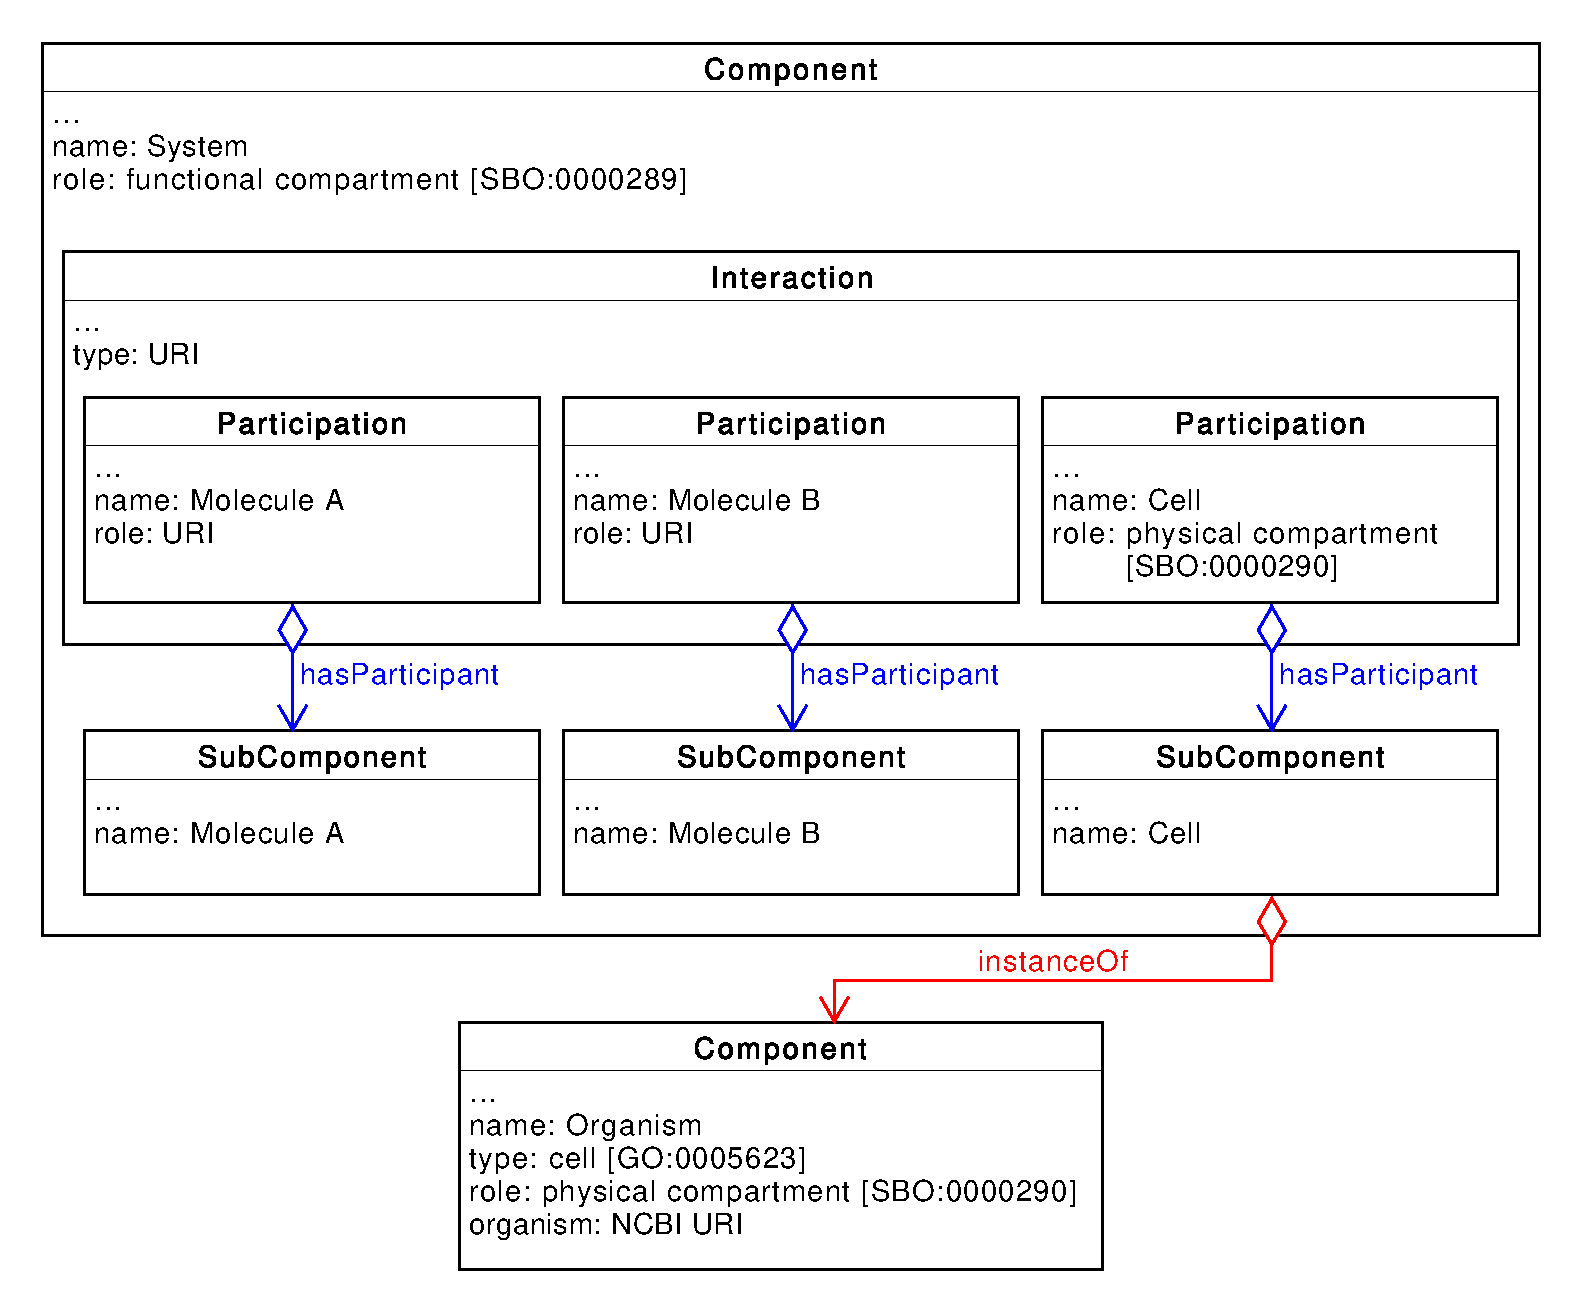
\includegraphics[width=\textwidth]{uml/cell_representation}
		\caption[Repressenting a cell]{This is a proposed approach for capturing cell designs in SBOL. A \sbol{Component} annotated with a URI pointing to an entry in the NCBI Taxonomy Database is used to capture information about the cell's strain/species. 
		The \sbol{Component} has a type of ``Cell'' from the Gene Ontology (GO), and a role of ``physical compartment''. 
		Another \sbol{Component} is used to represent a system in which the cell is implemented. 
		Entities, including the cell, are instantiated as \sbol{SubComponent}s, and process are captured using the \sbol{Interaction} class.
		Process which are contained within the cell are represented by including the cell as a participant with a role of ``physical compartment''. }
		\label{uml:cell_representation}
	\end{center}
\end{figure}

\subsubsection{Multiple Cells in a Single Design}

The same approach can be extended to represent systems with multiple cells, using one \sbol{Component} to represent the system for each cells.
The multicellular system can then be represented as a \sbol{Component} that includes the system description for each strain of cell as a \sbol{SubComponent}.
Interactions and constraints, such as a molecule that both strains interact with, are implemented using \sbol{ComponentReference}s to link to the definitions within each cell system description.
An example is shown in \ref{uml:multiple_cell_representation}.

\begin{figure}[ht]
	\begin{center}
		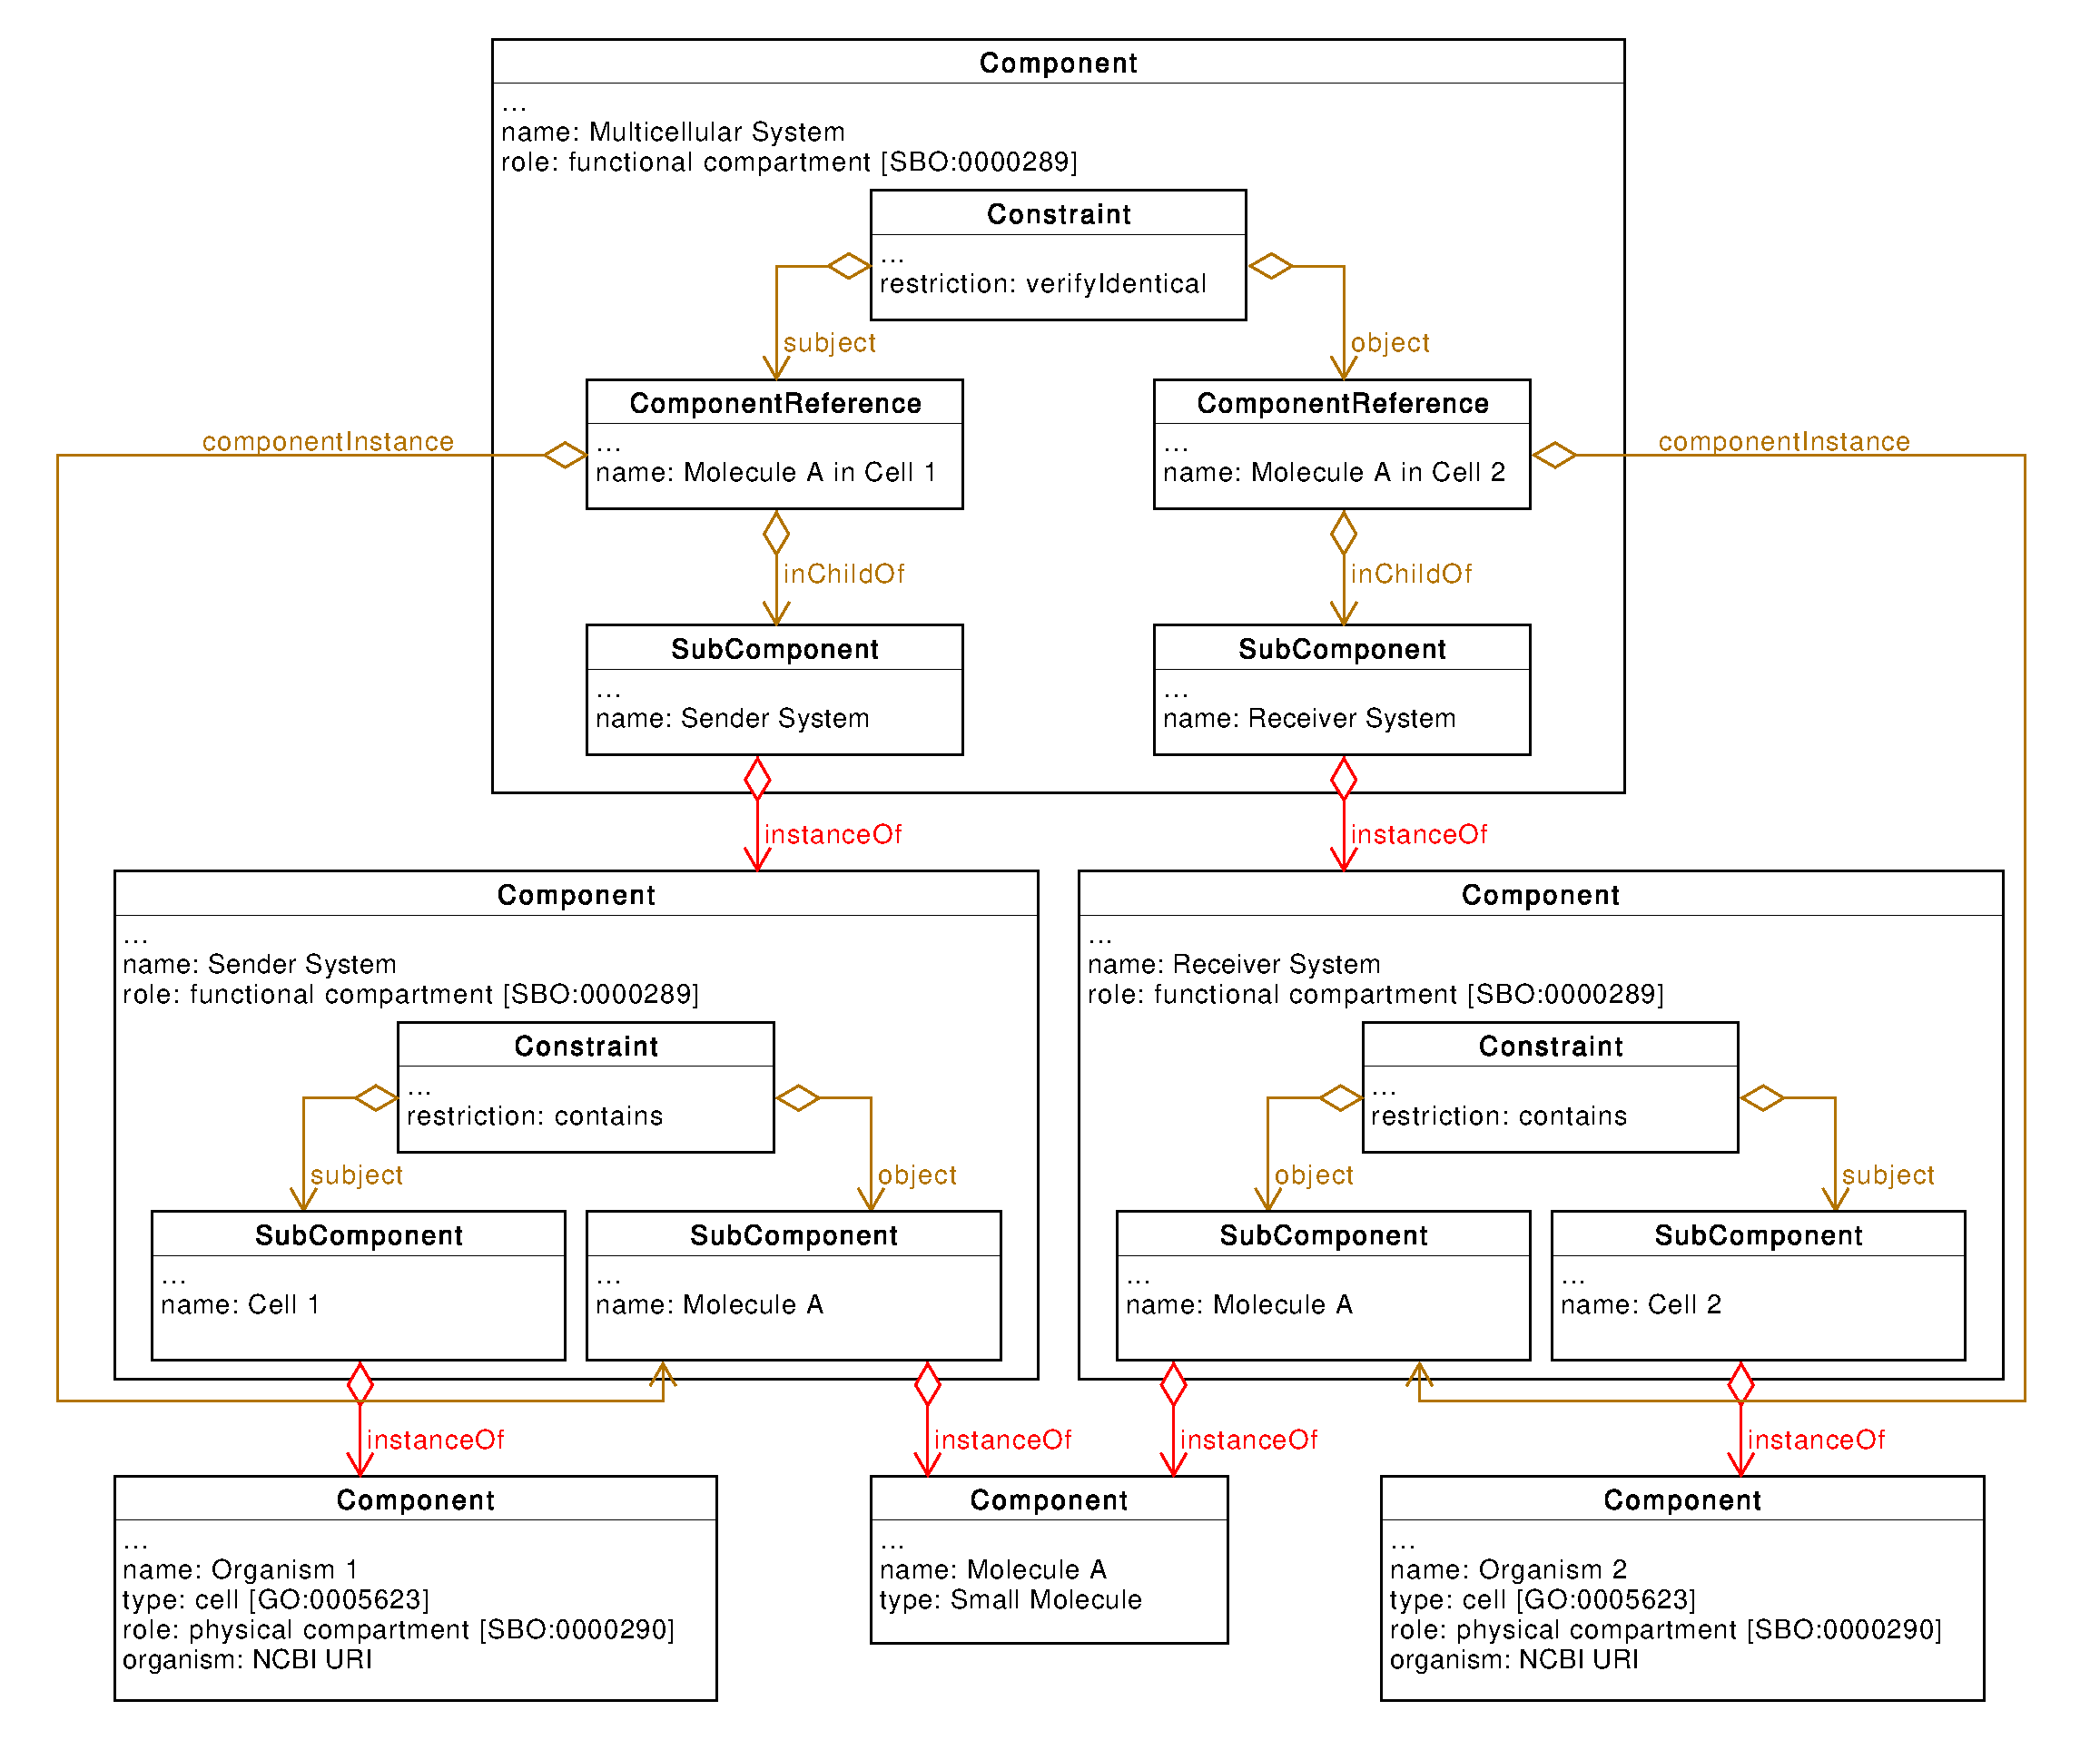
\includegraphics[width=\textwidth]{uml/two_cell_representation}
		\caption[]{Captured here is a design involving two cells which both interact with the small molecule ``Molecule A''. 
		Designs for the sender and receiver systems are captured using constraint to show that each of these cells interacts with the Molecule A contained within it.
		The overall multicellular system is represented by a \sbol{Component} with a \sbolmult{roles:C}{role} of ``functional compartment'', which is an SBO term.
		The two systems are included in this multicellular design as \sbol{SubComponent}s, and the fact that Molecule A is shared between systems is indicated with a constraint.}
		\label{uml:multiple_cell_representation}
	\end{center}
\end{figure}

\subsubsection{Cell Ratios}

The proportion of cell types present in a multicellular system can be captured using \sbol{Measure} on the representations of cells in the design.
As a best practice, the value of these measure classes is a percentage less than or equal to 100\%, representing the amount of a cell type present in the system compared to all other cell types present. 
Therefore, the sum of all these values specified in the system will typically be equal to 100\%, though this may not be the case if the system is not completely defined. 
An example is shown in \ref{uml:cell_ratios}.

\begin{figure}[ht]
	\begin{center}
		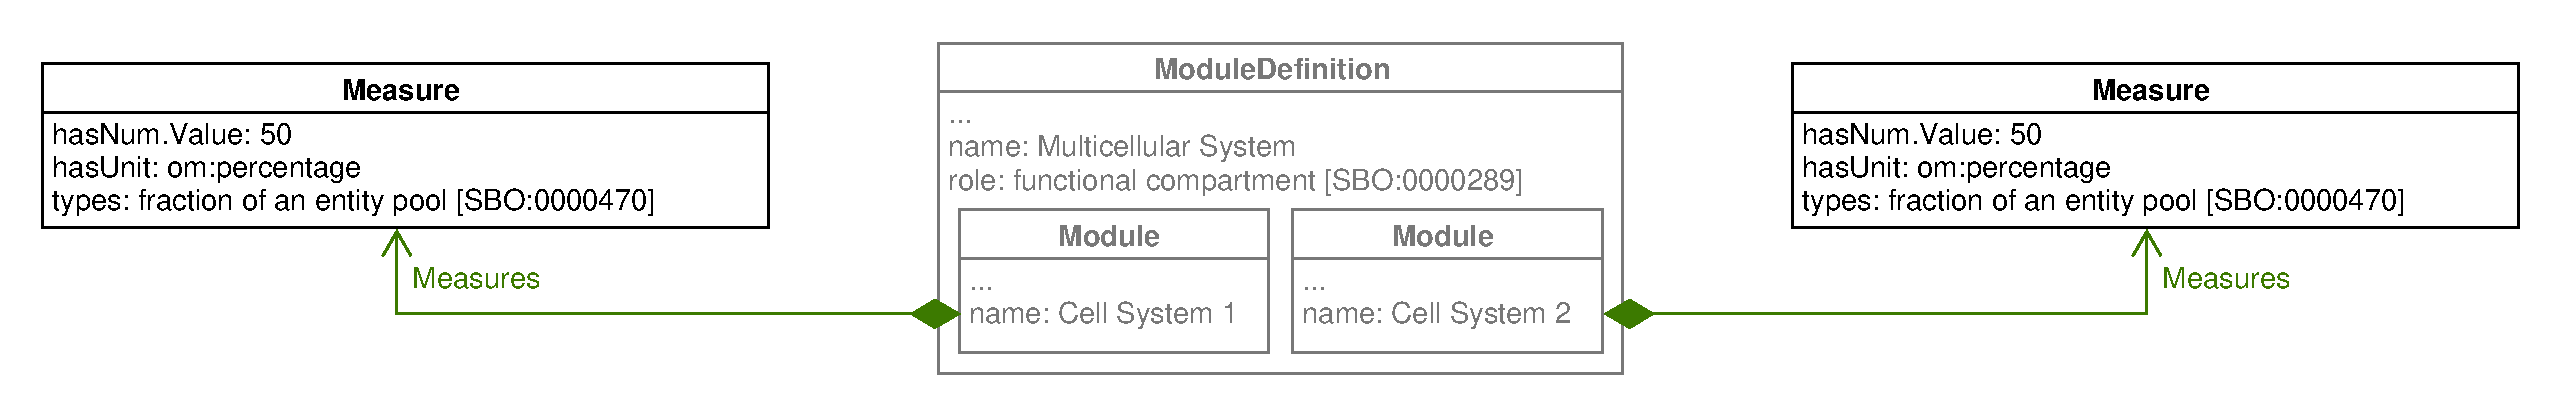
\includegraphics[width=\textwidth]{uml/cell_ratios}
		\caption[]{Annotating class instances with cellular proportions. Instances of the Measure class are used to capture the percentage of each cell type present in the multicellular system design.
		}
		\label{uml:cell_ratios}
	\end{center}
\end{figure}
